

\documentclass[11pt,fleqn]{book} % Default font size and left-justified equations

%%%%%%%%%%%%%%%%%%%%%%%%%%%%%%%%%%%%%%%%%
% The Legrand Orange Book
% Structural Definitions File
% Version 2.0 (9/2/15)
%
% Original author:
% Mathias Legrand (legrand.mathias@gmail.com) with modifications by:
% Vel (vel@latextemplates.com)
% 
% This file has been downloaded from:
% http://www.LaTeXTemplates.com
%
% License:
% CC BY-NC-SA 3.0 (http://creativecommons.org/licenses/by-nc-sa/3.0/)
%
%%%%%%%%%%%%%%%%%%%%%%%%%%%%%%%%%%%%%%%%%

%----------------------------------------------------------------------------------------
%	VARIOUS REQUIRED PACKAGES AND CONFIGURATIONS
%----------------------------------------------------------------------------------------

\usepackage[top=3cm,bottom=3cm,left=5.5cm,right=3cm,headsep=10pt,letterpaper,asymmetric]{geometry} % Page margins
% Could use 6cm margin on left 

\usepackage{graphicx} % Required for including pictures
\graphicspath{{Pictures/}} % Specifies the directory where pictures are stored

\usepackage{lipsum} % Inserts dummy text

\usepackage{tikz} % Required for drawing custom shapes

\usepackage[english]{babel} % English language/hyphenation

\usepackage{enumitem} % Customize lists
\setlist{noitemsep} % Reduce spacing between bullet points and numbered lists

\usepackage{booktabs} % Required for nicer horizontal rules in tables

\usepackage{xcolor} % Required for specifying colors by name
%\definecolor{rust}{RGB}{243,102,25} % Define the orange color used for highlighting throughout the book
\definecolor{rust}{RGB}{153, 0, 0} % Define alternate red color

\usepackage{pdftexcmds}



%----------------------------------------------------------------------------------------
%	FONTS
%----------------------------------------------------------------------------------------

\usepackage{avant} % Use the Avantgarde font for headings
%\usepackage{times} % Use the Times font for headings
\usepackage{mathptmx} % Use the Adobe Times Roman as the default text font together with math symbols from the Sym­bol, Chancery and Com­puter Modern fonts

\usepackage{microtype} % Slightly tweak font spacing for aesthetics
\usepackage[utf8]{inputenc} % Required for including letters with accents
\usepackage[T1]{fontenc} % Use 8-bit encoding that has 256 glyphs
\usepackage{relsize} % Allow relative font sizing
\renewcommand\RSlargest{100pt} 
%----------------------------------------------------------------------------------------
%	BIBLIOGRAPHY AND INDEX
%----------------------------------------------------------------------------------------

\usepackage[style=alphabetic,citestyle=numeric,sorting=nyt,sortcites=true,autopunct=true,babel=hyphen,hyperref=true,abbreviate=false,backref=true,backend=biber]{biblatex}
\addbibresource{bibliography.bib} % BibTeX bibliography file
\defbibheading{bibempty}{}

\usepackage{calc} % For simpler calculation - used for spacing the index letter headings correctly
\usepackage{makeidx} % Required to make an index
\makeindex % Tells LaTeX to create the files required for indexing

%----------------------------------------------------------------------------------------
%	MAIN TABLE OF CONTENTS
%----------------------------------------------------------------------------------------

\usepackage{titletoc} % Required for manipulating the table of contents

\contentsmargin{0cm} % Removes the default margin

% Part text styling
\titlecontents{part}[0cm]
{\addvspace{20pt}\centering\large\bfseries}
{}
{}
{}

% Chapter text styling
\titlecontents{chapter}[1.25cm] % Indentation
{\addvspace{12pt}\large\sffamily\bfseries} % Spacing and font options for chapters
{\color{rust!60}\contentslabel[\Large\thecontentslabel]{1.25cm}\color{rust}} % Chapter number
{\color{rust}}  
{\color{rust!60}\normalsize\;\titlerule*[.5pc]{.}\;\thecontentspage} % Page number

% Section text styling
\titlecontents{section}[1.25cm] % Indentation
{\addvspace{3pt}\sffamily\bfseries} % Spacing and font options for sections
{\contentslabel[\thecontentslabel]{1.25cm}} % Section number
{}
{\hfill\color{black}\thecontentspage} % Page number
[]

% Subsection text styling
\titlecontents{subsection}[1.25cm] % Indentation
{\addvspace{1pt}\sffamily\small} % Spacing and font options for subsections
{\contentslabel[\thecontentslabel]{1.25cm}} % Subsection number
{}
{\ \titlerule*[.5pc]{.}\;\thecontentspage} % Page number
[]

% List of figures
\titlecontents{figure}[0em]
{\addvspace{-5pt}\sffamily}
{\thecontentslabel\hspace*{1em}}
{}
{\ \titlerule*[.5pc]{.}\;\thecontentspage}
[]

% List of tables
\titlecontents{table}[0em]
{\addvspace{-5pt}\sffamily}
{\thecontentslabel\hspace*{1em}}
{}
{\ \titlerule*[.5pc]{.}\;\thecontentspage}
[]

%----------------------------------------------------------------------------------------
%	MINI TABLE OF CONTENTS IN PART HEADS
%----------------------------------------------------------------------------------------

% Chapter text styling
\titlecontents{lchapter}[0em] % Indenting
{\addvspace{15pt}\large\sffamily\bfseries} % Spacing and font options for chapters
{\color{rust}\contentslabel[\Large\thecontentslabel]{1.25cm}\color{rust}} % Chapter number
{}  
{\color{rust}\normalsize\sffamily\bfseries\;\titlerule*[.5pc]{.}\;\thecontentspage} % Page number

% Section text styling
\titlecontents{lsection}[0em] % Indenting
{\sffamily\small} % Spacing and font options for sections
{\contentslabel[\thecontentslabel]{1.25cm}} % Section number
{}
{}

% Subsection text styling
\titlecontents{lsubsection}[.5em] % Indentation
{\normalfont\footnotesize\sffamily} % Font settings
{}
{}
{}

%----------------------------------------------------------------------------------------
%	PAGE HEADERS
%----------------------------------------------------------------------------------------

\usepackage{fancyhdr} % Required for header and footer configuration

\pagestyle{fancy}
\renewcommand{\chaptermark}[1]{\markboth{\sffamily\normalsize\bfseries\chaptername\ \thechapter.\ #1}{}} % Chapter text font settings
\renewcommand{\sectionmark}[1]{\markright{\sffamily\normalsize\thesection\hspace{5pt}#1}{}} % Section text font settings
\fancyhf{} \fancyhead[LE,RO]{\sffamily\normalsize\thepage} % Font setting for the page number in the header
\fancyhead[LO]{\rightmark} % Print the nearest section name on the left side of odd pages
\fancyhead[RE]{\leftmark} % Print the current chapter name on the right side of even pages
\renewcommand{\headrulewidth}{0.5pt} % Width of the rule under the header
\addtolength{\headheight}{2.5pt} % Increase the spacing around the header slightly
\renewcommand{\footrulewidth}{0pt} % Removes the rule in the footer
\fancypagestyle{plain}{\fancyhead{}\renewcommand{\headrulewidth}{0pt}} % Style for when a plain pagestyle is specified

% Removes the header from odd empty pages at the end of chapters
\makeatletter
\renewcommand{\cleardoublepage}{
\clearpage\ifodd\c@page\else
\hbox{}
\vspace*{\fill}
\thispagestyle{empty}
\newpage
\fi}

%----------------------------------------------------------------------------------------
%	THEOREM STYLES
%----------------------------------------------------------------------------------------

\usepackage{amsmath,amsfonts,amssymb,amsthm} % For math equations, theorems, symbols, etc

\newcommand{\intoo}[2]{\mathopen{]}#1\,;#2\mathclose{[}}
\newcommand{\ud}{\mathop{\mathrm{{}d}}\mathopen{}}
\newcommand{\intff}[2]{\mathopen{[}#1\,;#2\mathclose{]}}
\newtheorem{notation}{Notation}[chapter]

% Boxed/framed environments
\newtheoremstyle{rustnumbox}% % Theorem style name
{0pt}% Space above
{0pt}% Space below
{\normalfont}% % Body font
{}% Indent amount
{\small\bf\sffamily\color{rust}}% % Theorem head font
{\;}% Punctuation after theorem head
{0.25em}% Space after theorem head
{\small\sffamily\color{rust}\thmname{#1}\nobreakspace\thmnumber{\@ifnotempty{#1}{}\@upn{#2}}% Theorem text (e.g. Theorem 2.1)
\thmnote{\nobreakspace\the\thm@notefont\sffamily\bfseries\color{black}---\nobreakspace#3.}} % Optional theorem note
\renewcommand{\qedsymbol}{$\blacksquare$}% Optional qed square

\newtheoremstyle{blacknumex}% Theorem style name
{5pt}% Space above
{5pt}% Space below
{\normalfont}% Body font
{} % Indent amount
{\small\bf\sffamily}% Theorem head font
{\;}% Punctuation after theorem head
{0.25em}% Space after theorem head
{\small\sffamily{\tiny\ensuremath{\blacksquare}}\nobreakspace\thmname{#1}\nobreakspace\thmnumber{\@ifnotempty{#1}{}\@upn{#2}}% Theorem text (e.g. Theorem 2.1)
\thmnote{\nobreakspace\the\thm@notefont\sffamily\bfseries---\nobreakspace#3.}}% Optional theorem note

\newtheoremstyle{blacknumbox} % Theorem style name
{0pt}% Space above
{0pt}% Space below
{\normalfont}% Body font
{}% Indent amount
{\small\bf\sffamily}% Theorem head font
{\;}% Punctuation after theorem head
{0.25em}% Space after theorem head
{\small\sffamily\thmname{#1}\nobreakspace\thmnumber{\@ifnotempty{#1}{}\@upn{#2}}% Theorem text (e.g. Theorem 2.1)
\thmnote{\nobreakspace\the\thm@notefont\sffamily\bfseries---\nobreakspace#3.}}% Optional theorem note

% Non-boxed/non-framed environments
\newtheoremstyle{rustnum}% % Theorem style name
{5pt}% Space above
{5pt}% Space below
{\normalfont}% % Body font
{}% Indent amount
{\small\bf\sffamily\color{rust}}% % Theorem head font
{\;}% Punctuation after theorem head
{0.25em}% Space after theorem head
{\small\sffamily\color{rust}\thmname{#1}\nobreakspace\thmnumber{\@ifnotempty{#1}{}\@upn{#2}}% Theorem text (e.g. Theorem 2.1)
\thmnote{\nobreakspace\the\thm@notefont\sffamily\bfseries\color{black}---\nobreakspace#3.}} % Optional theorem note
\renewcommand{\qedsymbol}{$\blacksquare$}% Optional qed square
\makeatother

% Defines the theorem text style for each type of theorem to one of the three styles above
\newcounter{dummy} 
\numberwithin{dummy}{section}
\theoremstyle{rustnumbox}
\newtheorem{theoremeT}[dummy]{Theorem}
\newtheorem{assignment}{Assignment}[chapter]

\newtheorem{exerciseT}{Exercise}[chapter]
\theoremstyle{blacknumex}
\newtheorem{exampleT}{Example}[chapter]
\theoremstyle{blacknumbox}
\newtheorem{vocabulary}{Vocabulary}[chapter]
\newtheorem{definitionT}{Definition}[section]
\newtheorem{corollaryT}[dummy]{Corollary}
\theoremstyle{rustnum}
\newtheorem{proposition}[dummy]{Proposition}

%----------------------------------------------------------------------------------------
%	DEFINITION OF COLORED BOXES
%----------------------------------------------------------------------------------------

\RequirePackage[framemethod=default]{mdframed} % Required for creating the theorem, definition, exercise and corollary boxes

% Theorem box
\newmdenv[skipabove=7pt,
skipbelow=7pt,
backgroundcolor=black!5,
linecolor=rust,
innerleftmargin=5pt,
innerrightmargin=5pt,
innertopmargin=5pt,
leftmargin=0cm,
rightmargin=0cm,
innerbottommargin=5pt]{tBox}

% Exercise box	  
\newmdenv[skipabove=7pt,
skipbelow=7pt,
rightline=false,
leftline=true,
topline=false,
bottomline=false,
backgroundcolor=rust!10,
linecolor=rust,
innerleftmargin=5pt,
innerrightmargin=5pt,
innertopmargin=5pt,
innerbottommargin=5pt,
leftmargin=0cm,
rightmargin=0cm,
linewidth=4pt]{eBox}	

% Definition box
\newmdenv[skipabove=7pt,
skipbelow=7pt,
rightline=false,
leftline=true,
topline=false,
bottomline=false,
linecolor=rust,
innerleftmargin=5pt,
innerrightmargin=5pt,
innertopmargin=0pt,
leftmargin=0cm,
rightmargin=0cm,
linewidth=4pt,
innerbottommargin=0pt]{dBox}	

% Corollary box
\newmdenv[skipabove=7pt,
skipbelow=7pt,
rightline=false,
leftline=true,
topline=false,
bottomline=false,
linecolor=gray,
backgroundcolor=black!5,
innerleftmargin=5pt,
innerrightmargin=5pt,
innertopmargin=5pt,
leftmargin=0cm,
rightmargin=0cm,
linewidth=4pt,
innerbottommargin=5pt]{cBox}

% Creates an environment for each type of theorem and assigns it a theorem text style from the "Theorem Styles" section above and a colored box from above
\newenvironment{theorem}{\begin{tBox}\begin{theoremeT}}{\end{theoremeT}\end{tBox}}
\newenvironment{exercise}{\begin{eBox}\begin{exerciseT}}{\hfill{\color{rust}\tiny\ensuremath{\blacksquare}}\end{exerciseT}\end{eBox}}				  
\newenvironment{definition}{\begin{dBox}\begin{definitionT}}{\end{definitionT}\end{dBox}}	
\newenvironment{example}{\begin{exampleT}}{\hfill{\tiny\ensuremath{\blacksquare}}\end{exampleT}}		
\newenvironment{corollary}{\begin{cBox}\begin{corollaryT}}{\end{corollaryT}\end{cBox}}	

%----------------------------------------------------------------------------------------
%	WARNING ENVIRONMENT
%----------------------------------------------------------------------------------------

\newenvironment{warning}{\par\vspace{10pt}\small % Vertical white space above the remark and smaller font size
	\begin{list}{}{
			\leftmargin=35pt % Indentation on the left
			\rightmargin=25pt}\item\ignorespaces % Indentation on the right
		\makebox[-2.5pt]{\begin{tikzpicture}[overlay]
			\node[draw=rust!60,line width=1pt,circle,fill=rust!25,font=\sffamily\bfseries,inner sep=2pt,outer sep=0pt] at (-15pt,0pt){\textcolor{rust}{\textbf{!}}};\end{tikzpicture}} 
		\advance\baselineskip -1pt}{\end{list}\vskip5pt} % Tighter line spacing and white space after remark

%----------------------------------------------------------------------------------------
%	REMARK ENVIRONMENT
%----------------------------------------------------------------------------------------

\newenvironment{remark}{\par\vspace{10pt}\small % Vertical white space above the remark and smaller font size
\begin{list}{}{
\leftmargin=35pt % Indentation on the left
\rightmargin=25pt}\item\ignorespaces % Indentation on the right
\makebox[-2.5pt]{\begin{tikzpicture}[overlay]
\node[draw=rust!60,line width=1pt,circle,fill=rust!25,font=\sffamily\bfseries,inner sep=2pt,outer sep=0pt] at (-15pt,0pt){\textcolor{rust}{R}};\end{tikzpicture}} % Orange R in a circle
\advance\baselineskip -1pt}{\end{list}\vskip5pt} % Tighter line spacing and white space after remark

%----------------------------------------------------------------------------------------
%	SECTION NUMBERING IN THE MARGIN
%----------------------------------------------------------------------------------------

\makeatletter

% just bottom line
%\newmdenv[topline=false,leftline=false,rightline=false]{test123}

%\newmdenv[
%rightline=false, leftline=false, topline=false, bottomline=true,
%linecolor=rust, linewidth=4pt
%]{sectionUnderline}

% Adjusts all numbering for sections and subsections
\renewcommand{\@seccntformat}[1]{  
    \ifnum\pdf@strcmp{#1}{section}=\z@ 
    
    %\llap{\colorbox{gray!15}{\makebox[3.25cm][r]{\textcolor{gray}{\textsc{\@nameuse{secTypeName}}\hspace{0.5em}\relsize{1.25}\textcolor{rust}{\csname the#1\endcsname}}}}\hspace{.5em}}
    \llap{
        %\begin{sectionUnderline}
            \makebox[3.25cm][r]{\textcolor{gray}{\textsc{\@nameuse{secTypeName}}\hspace{0.5em}\relsize{1.25}\textcolor{rust}{\csname the#1\endcsname}}}
            \textcolor{rust}{\hspace{-3.25cm}\rule[-.2cm]{3.13cm}{2pt}}
        %\end{sectionUnderline}
        \hspace{.5em}
    }
    \else
    \llap{\textcolor{rust}{\csname the#1\endcsname}\hspace{1em}}%
    \fi 
   % \llap{\textcolor{rust}{\csname the#1\endcsname}\hspace{1em}}
}  % hspace controls spacing of section number to section name    


\newcommand{\setSectionType}[1]{
    \@namedef{secTypeName}{#1}
}
        
\renewcommand{\section}{\@startsection{section}{1}{-8pt}
{-5ex \@plus -1ex \@minus -.2ex}
{2.0ex \@plus.2ex }
{\normalfont\large\sffamily\bfseries}}


\renewcommand{\subsection}{\@startsection {subsection}{2}{-3pt}
{-3ex \@plus -0.1ex \@minus -.4ex}
{0.5ex \@plus.2ex }
{\normalfont\sffamily\bfseries}}
\renewcommand{\subsubsection}{\@startsection {subsubsection}{3}{\z@}
{-2ex \@plus -0.1ex \@minus -.2ex}
{.2ex \@plus.2ex }
{\normalfont\small\sffamily\bfseries}}                        
\renewcommand\paragraph{\@startsection{paragraph}{4}{\z@}
{-2ex \@plus-.2ex \@minus .2ex}
{.1ex}
{\normalfont\small\sffamily\bfseries}}

%----------------------------------------------------------------------------------------
%	PART HEADINGS
%----------------------------------------------------------------------------------------

% numbered part in the table of contents
\newcommand{\@mypartnumtocformat}[2]{%
\setlength\fboxsep{0pt}%
\noindent\colorbox{rust!20}{\strut\parbox[c][.7cm]{\ecart}{\color{rust!70}\Large\sffamily\bfseries\centering#1}}\hskip\esp\colorbox{rust!40}{\strut\parbox[c][.7cm]{\linewidth-\ecart-\esp}{\Large\sffamily\centering#2}}}%
%%%%%%%%%%%%%%%%%%%%%%%%%%%%%%%%%%
% unnumbered part in the table of contents
\newcommand{\@myparttocformat}[1]{%
\setlength\fboxsep{0pt}%
\noindent\colorbox{rust!40}{\strut\parbox[c][.7cm]{\linewidth}{\Large\sffamily\centering#1}}}%
%%%%%%%%%%%%%%%%%%%%%%%%%%%%%%%%%%
\newlength\esp
\setlength\esp{4pt}
\newlength\ecart
\setlength\ecart{1.2cm-\esp}
\newcommand{\thepartimage}{}%
\newcommand{\partimage}[1]{\renewcommand{\thepartimage}{#1}}%
\def\@part[#1]#2{%
\ifnum \c@secnumdepth >-2\relax%
\refstepcounter{part}%
\addcontentsline{toc}{part}{\texorpdfstring{\protect\@mypartnumtocformat{\thepart}{#1}}{\partname~\thepart\ ---\ #1}}
\else%
\addcontentsline{toc}{part}{\texorpdfstring{\protect\@myparttocformat{#1}}{#1}}%
\fi%
\startcontents%
\markboth{}{}%
{\thispagestyle{empty}%
\begin{tikzpicture}[remember picture,overlay]%
\node at (current page.north west){\begin{tikzpicture}[remember picture,overlay]%	
\node[anchor=north] at (4cm,-3.25cm){\color{rust!60}\fontsize{220}{100}\sffamily\bfseries\@Roman\c@part}; 
\node[anchor=south east] at (\paperwidth-1cm,-\paperheight+1cm){\parbox[t][][t]{8.5cm}{
\printcontents{l}{0}{\setcounter{tocdepth}{1}}%
}};
\node[anchor=north east] at (\paperwidth-1.5cm,-3.25cm){\parbox[t][][t]{15cm}{\strut\raggedleft\color{black!40}\fontsize{30}{30}\sffamily\bfseries#2}};
\end{tikzpicture}};
\end{tikzpicture}}%
\@endpart}
\def\@spart#1{%
\startcontents%
\phantomsection
{\thispagestyle{empty}%
\begin{tikzpicture}[remember picture,overlay]%
\node at (current page.north west){\begin{tikzpicture}[remember picture,overlay]%	
\fill[rust!20](0cm,0cm) rectangle (\paperwidth,-\paperheight);
\node[anchor=north east] at (\paperwidth-1.5cm,-3.25cm){\parbox[t][][t]{15cm}{\strut\raggedleft\color{white}\fontsize{30}{30}\sffamily\bfseries#1}};
\end{tikzpicture}};
\end{tikzpicture}}
\addcontentsline{toc}{part}{\texorpdfstring{%
\setlength\fboxsep{0pt}%
\noindent\protect\colorbox{rust!40}{\strut\protect\parbox[c][.7cm]{\linewidth}{\Large\sffamily\protect\centering #1\quad\mbox{}}}}{#1}}%
\@endpart}
\def\@endpart{\vfil\newpage
\if@twoside
\if@openright
\null
\thispagestyle{empty}%
\newpage
\fi
\fi
\if@tempswa
\twocolumn
\fi}

%----------------------------------------------------------------------------------------
%	CHAPTER HEADINGS
%----------------------------------------------------------------------------------------

% A switch to conditionally include a picture, implemented by  Christian Hupfer
\newif\ifusechapterimage
\usechapterimagetrue
\newcommand{\thechapterimage}{}%
\newcommand{\chapterimage}[1]{\ifusechapterimage\renewcommand{\thechapterimage}{#1}\fi}%
\def\@makechapterhead#1{%
{\parindent \z@ \raggedright \normalfont
\ifnum \c@secnumdepth >\m@ne
\if@mainmatter
\begin{tikzpicture}[remember picture,overlay]
\node at (current page.north west)
{\begin{tikzpicture}[remember picture,overlay]
\node[anchor=north west,inner sep=0pt] at (0,0) {\ifusechapterimage\includegraphics[width=\paperwidth]{\thechapterimage}\fi};
%\draw[anchor=west] (\Gm@lmargin,-9cm) node [line width=2pt,rounded corners=15pt,draw=rust,fill=white,fill opacity=0.5,inner sep=15pt]{\strut\makebox[22cm]{}};

%%%%% Chapter text sizing
%\draw[anchor=west] (\Gm@lmargin-1.3cm,-4cm) node [line width=2pt,rounded corners=15pt,draw=rust,fill=white,fill opacity=0.75,inner sep=15pt]{\strut\makebox[22cm]{}};

%\draw[anchor=west] (\Gm@lmargin-1cm,-4.1cm) node {\huge\sffamily\bfseries\color{black}\thechapter. #1\strut};

% Use larger chapter number

\draw[anchor=west] (\Gm@lmargin-1.3cm,-3.9cm) node [line width=2pt,rounded corners=8pt,draw=rust,fill=white,fill opacity=0.75,inner sep=15pt]{\strut\makebox[22cm]{}};

\draw[anchor=west] (\Gm@lmargin-1cm,-4.0cm) node {\huge\sffamily\bfseries\color{black}{\relsize{2}\thechapter. }#1\strut};


\end{tikzpicture}};
\end{tikzpicture}
\else
\begin{tikzpicture}[remember picture,overlay]
\node at (current page.north west)
{\begin{tikzpicture}[remember picture,overlay]
\node[anchor=north west,inner sep=0pt] at (0,0) {\ifusechapterimage\includegraphics[width=\paperwidth]{\thechapterimage}\fi};
%\draw[anchor=west] (\Gm@lmargin,-9cm) node [line width=2pt,rounded corners=15pt,draw=rust,fill=white,fill opacity=0.5,inner sep=15pt]{\strut\makebox[22cm]{}};

\draw[anchor=west] (\Gm@lmargin,-4cm) node [line width=2pt,rounded corners=15pt,draw=rust,fill=white,fill opacity=0.75,inner sep=15pt]{\strut\makebox[22cm]{}};

\draw[anchor=west] (\Gm@lmargin+.3cm,-4cm) node {\huge\sffamily\bfseries\color{black}#1\strut};
\end{tikzpicture}};
\end{tikzpicture}
%\fi\fi\par\vspace*{270\p@}}}

\fi\fi\par\vspace*{150\p@}}}

%-------------------------------------------

\def\@makeschapterhead#1{%
\begin{tikzpicture}[remember picture,overlay]
\node at (current page.north west)
{\begin{tikzpicture}[remember picture,overlay]
\node[anchor=north west,inner sep=0pt] at (0,0) {\ifusechapterimage\includegraphics[width=\paperwidth]{\thechapterimage}\fi};
\draw[anchor=west] (\Gm@lmargin,-9cm) node [line width=2pt,rounded corners=15pt,draw=rust,fill=white,fill opacity=0.5,inner sep=15pt]{\strut\makebox[22cm]{}};
\draw[anchor=west] (\Gm@lmargin+.3cm,-9cm) node {\huge\sffamily\bfseries\color{black}#1\strut};
\end{tikzpicture}};
\end{tikzpicture}
\par\vspace*{270\p@}}
\makeatother

%----------------------------------------------------------------------------------------
%	HYPERLINKS IN THE DOCUMENTS
%----------------------------------------------------------------------------------------

\usepackage{hyperref}
\hypersetup{hidelinks,backref=true,pagebackref=true,hyperindex=true,colorlinks=false,breaklinks=true,urlcolor= rust,bookmarks=true,bookmarksopen=false,pdftitle={Lab Manual},pdfauthor={Brent Mellor}}
\usepackage{bookmark}
\bookmarksetup{
open,
numbered,
addtohook={%
\ifnum\bookmarkget{level}=0 % chapter
\bookmarksetup{bold}%
\fi
\ifnum\bookmarkget{level}=-1 % part
\bookmarksetup{color=rust,bold}%
\fi
}
}
 % Insert the commands.tex file which contains the majority of the structure behind the template
\usepackage{float}

\usepackage{listings} 
\lstset
{ 
    language=C,
    basicstyle=\ttfamily,
    columns=fullflexible,
    keepspaces=true,
    numbers=none,
    stepnumber=1,
    showstringspaces=false,
    tabsize=1,
    breaklines=true,
    breakatwhitespace=false,
    keywordstyle=\color{blue!80!black},
    stringstyle=\color{red!80!black},
    commentstyle=\color{green!40!black},
    morecomment=[l][\color{magenta!80!black}]{\#}
}

\usepackage{caption}
\captionsetup[figure]{font=small,skip=10pt}

%\usepackage{enumitem}
%\setlist{noitemsep} % or \setlist{noitemsep} to leave space around whole list


%%%%% May be too harsh to prevent paragraph breaks across pages! 
%\interlinepenalty 10000
\widowpenalties 1 10000
\raggedbottom


\newcommand{\ilcode}[1]{
    %\vspace{0.5pt}
    \smallskip
    \colorbox{gray!20!white}{
        \centering
        \parbox{\linewidth-2\fboxsep}{
            \lstinline@#1@
        }
    }
    %\vspace{0.5pt}
}

\newcommand{\code}[3]{
    \begin{figure}[]
        \colorbox{gray!20!white}{
            \parbox{\linewidth-2\fboxsep} {
                \centering 
                \lstinputlisting[language=C]{#1}
            }
        }
        \caption{#2}
        \label{#3}
    \end{figure}
}

\usepackage{textcomp}
\usepackage{wrapfig}
\usepackage{float}

\usepackage{silence} % http://ctan.org/pkg/silence
\ErrorFilter{textcomp}{Symbol \textrightarrow not provided}

% Disable paragraph indentation globally since template was indenting some and not others. (looked terrible)
\setlength{\parindent}{0pt}


%%%%%%%%%%%%%%%%%%%%%%%%%%%%%%%%%%%%%%%%%%%%%%%%%%%%%%%%%%%%%%%%%%%%%%%%%%%%%%%%%%%%%%%%%%%%%%%%%
%%%%                                                                                         %%%%
%%%%       Chapter 7:                                                                        %%%%
%%%%                                                                                         %%%%
%%%%%%%%%%%%%%%%%%%%%%%%%%%%%%%%%%%%%%%%%%%%%%%%%%%%%%%%%%%%%%%%%%%%%%%%%%%%%%%%%%%%%%%%%%%%%%%%%

\setcounter{chapter}{6} % Manually adjust chapter counter to number before desired chapter heading

\begin{document}
	
\chapterimage{chapter_head_2.png} % Chapter heading image
\chapter{Analog Signals and the ADC/DAC}

%\begin{warning}
%    This lab manual is an early revision, the content will change as it is improved and expanded. 
%\end{warning}

\section{The Analog Truth Behind Digital Signals}
All of the signals we have been dealing with in the previous labs have been digital, in that we've been considering them as either "high" or "low". However all real-world signals are actually analog. Regardless of how cleanly and crisp a signal is when generated, it is essentially a voltage on a wire with an analog value such as 3V or 0V. As digital signals travel their sharp edged transitions soften and blur. Often, external factors introduce signal noise in the form of voltage instability/ripple or spikes and dips.

Because of this, digital inputs contain circuitry to recover the original digital meaning from the messy analog signal received. The simplest method of recovering a digital signal is using a voltage threshold. Any voltage greater than the threshold value is considered a digital high, anything less than the threshold is a digital low. 

Thresholding only works well when the input signal is relatively clean and avoids values near the threshold. An input signal with voltages close to the threshold have the tendency to cause rapid transitions since even small noise ripples can move the value above and below the trigger point. An improvement on simple thresholding is to use \textit{hysteresis}. 

\subsubsection{Hysteresis}

Hysteresis changes the voltage threshold depending on the currently detected digital state. This makes it impossible for a signal to consistently hang around the trigger point. For example, once a signal is interpreted as digital high, the threshold for transitioning to digital low moves downwards, and requires a very low value to move to the low state. Even if the analog value remains near the original threshold voltage for detecting a logic high signal, small ripples won't cause unwanted transitions since the threshold moved. One commonly used hysteresis circuit is known as a \textit{Schmidt Trigger}. Figure \ref{schmidt} shows the schematic symbol for a Schmidt Trigger and its operation. Signal `U' is the analog input to be converted into digital signals. Signal `A' shows the output of a simple threshold indicated by a dashed red line. Signal `B' shows the output of a system with hysteresis, the two positions of the moving threshold are indicated by green dashed lines. 

\begin{figure}[]
    \centering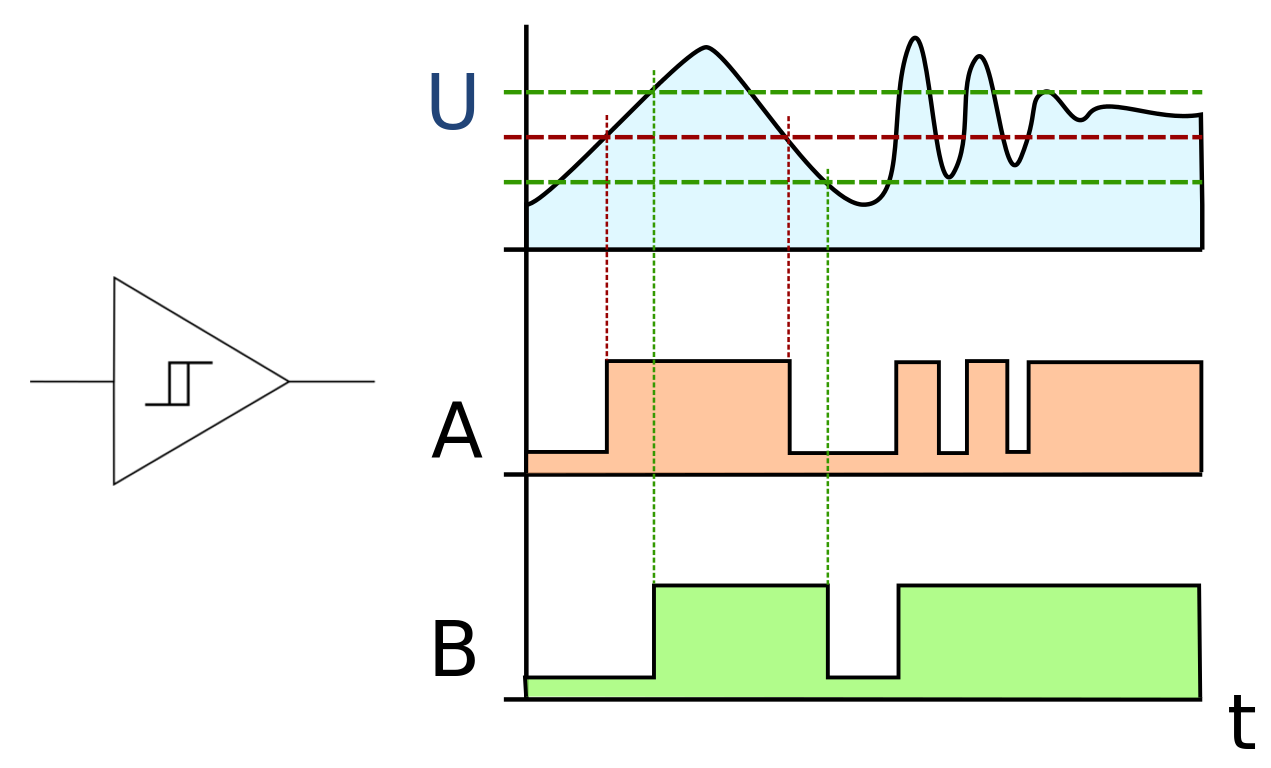
\includegraphics[width=.75\textwidth]{schmidt}
    \caption{Symbol and operation of a Schmidt Trigger.}
    \label{schmidt}
\end{figure}

\subsubsection{Simple Analog Waveforms}
Many everyday devices use analog signals. Common examples include: sensors, speakers, motors, and the AC power in the wall. Some analog signals such as a battery have very simple and (hopefully) predictable characteristics. Others such as audio, have complex waves which are non-repetitive and consist of combinations of many frequencies. For this lab we'll be working with a few of the fundamental wave shapes: sinusoidal, triangle, sawtooth and square. Figure \ref{waves} shows examples of each of these. 

\begin{figure}[]
    \centering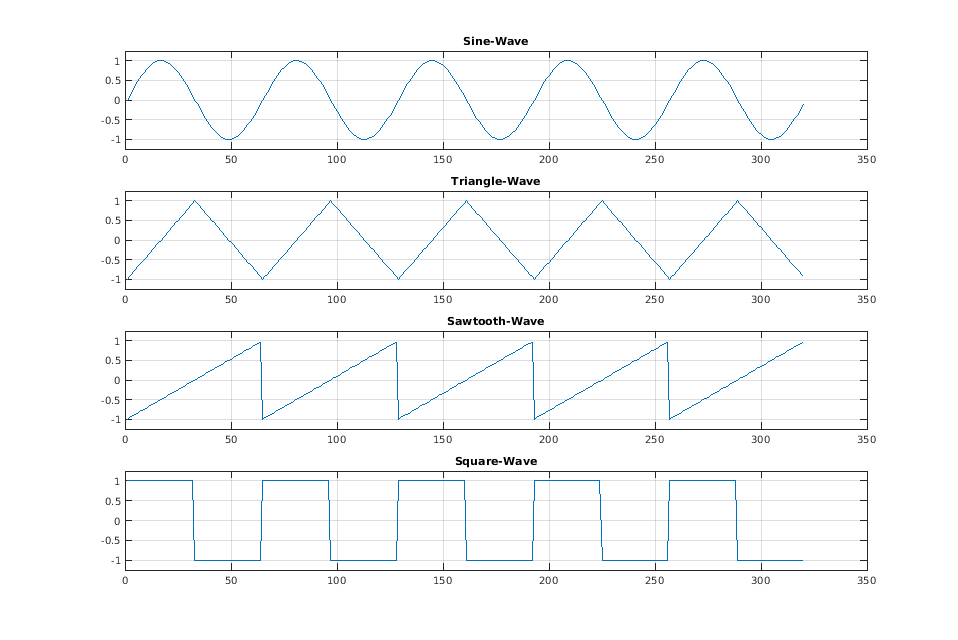
\includegraphics[width=0.8\textwidth]{waves}
    \caption{Fundamental wave shapes.}
    \label{waves}
\end{figure}


\section{Representing Analog Signals Digitally}
When interpreting an analog signal directly as a high/low digital signal, basic hysteresis circuits such as a Schmidt trigger are sufficient. However, many systems such as sensors, produce analog signals where the specific voltage of the output represents information. For these signals we must use dedicated hardware that can represent a voltage range as a sequence of binary numbers. Unfortunately, the conversion between analog and digital is never perfect and there are a few limitations and sources of error you need to understand. 

Since this isn't a digital signal processing class, we'll be covering just the barest minimum of theory required to understand the following concepts.

\subsection{Quantization}
Converting analog to digital is similar to setting up a range of increasing threshold values and counting how many the input signal crosses. Because of this, the fewer threshold values there are, the more granular the result and less information received about the input signal. This is the basis of \textit{quantization}.

Quantization is the process of mapping a high-resolution signal to a manageable lower-resolution one. Analog signals technically have infinite resolution in their voltage levels, we would like to represent groups of these voltages as a range of digital numbers. Digital quantization is represented by the number of binary bits in its output, a 2-bit device has four values, an 8-bit system can represent 256. 

When quantizing a signal you take the maximal range of the input and split it into a number of chunks (placing thresholds) determined by the range that the output supports. Basically, quantization "flattens" pieces of the input signal to make it representable in a certain number range. Figure \ref{quantization} shows a (red) analog sine wave being \textit{quantized} into a (blue) 2-bit range or four level digital representation.  


\subsubsection{Quantization Error}
The main issue quantizing signals is that their value will always be in a state where the input value is higher than the last triggered threshold, but not high enough to trigger the next. Unfortunately, changes within an input signal are lost unless they are large enough to cross one of the threshold values. This concept is the basis of quantization error. 

Quantization error describes the difference between the real analog input and the quantized output values. The larger each quantization step, the larger the error grows before the output changes to the next value and becomes closer to the input's true value. 

Figure \ref{quantized_sine} shows a sine-wave converted into a range of quantization resolutions. As the number of output bits increases, the number of possible voltage steps increases. As the number of steps increase, the difference in voltage between them becomes smaller. As the voltage differences decrease we are able to represent more accurately the real analog value at that point in time.

\begin{figure}[]
    \centering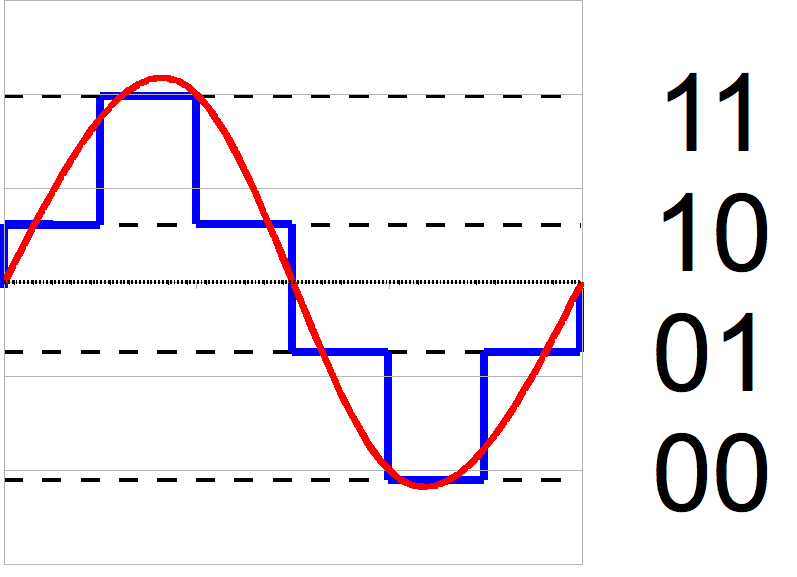
\includegraphics[width=.4\textwidth]{quantization}
    \caption{2-bit quantized sine-wave cycle.}
    \label{quantization}
\end{figure}

\begin{figure}[]
    \centering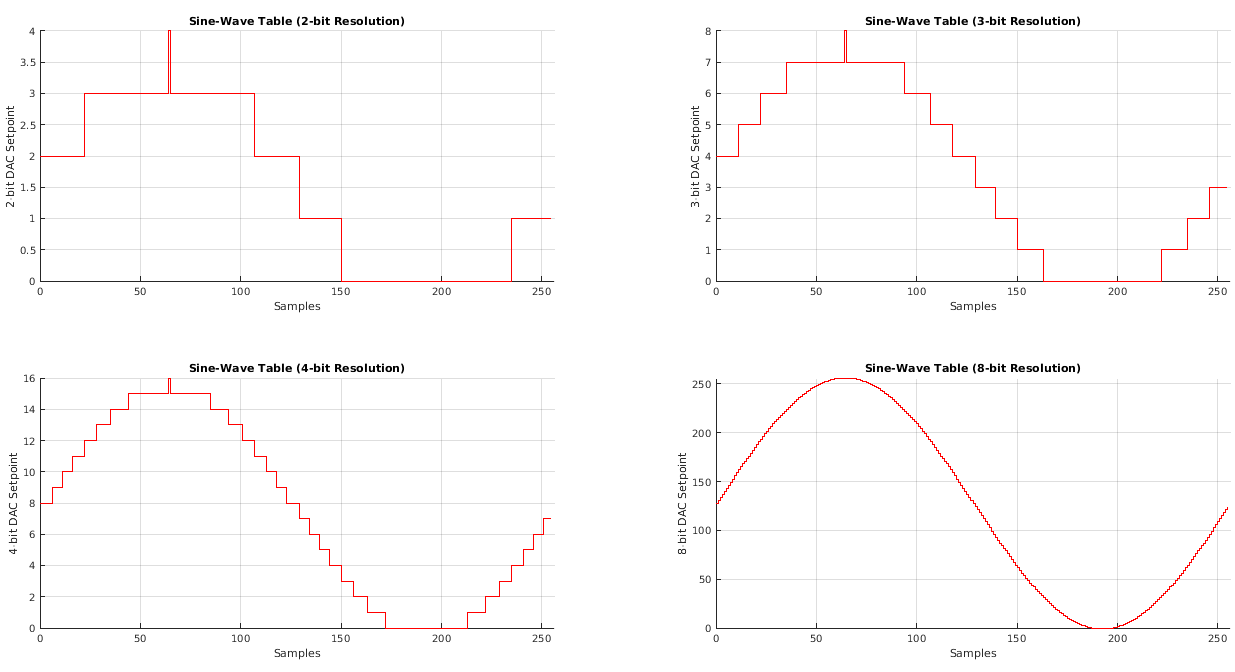
\includegraphics[width=\textwidth]{quantized_sine}
    \caption{Sine-wave cycle under different quantization levels.}
    \label{quantized_sine}
\end{figure}

\subsection{Sampling Rate and Nyquist Theory}
Unfortunately the number of voltage steps isn't the only thing we have to worry about when converting between analog and digital. Figure \ref{nyquist}, shows that at every sampling point of the analog signals, both of the two different waves shown have the same value. This problem is the core of something called Nyquist theory.

\begin{figure}[]
    \centering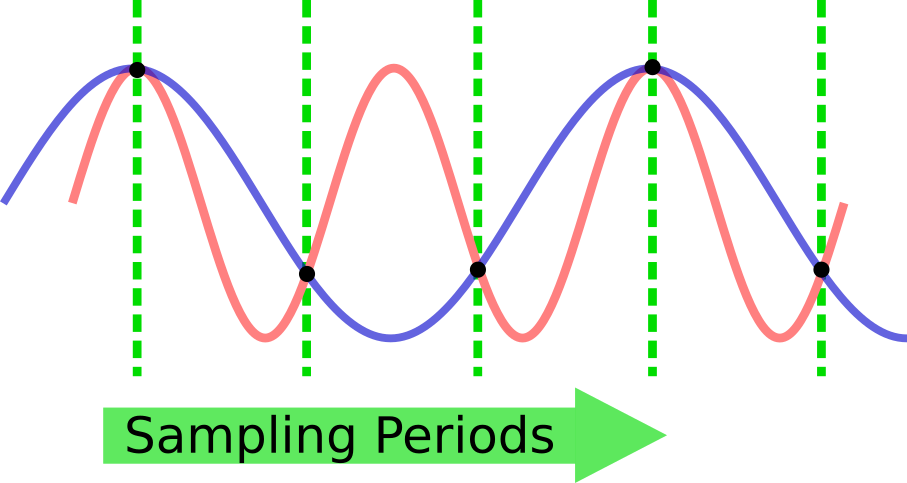
\includegraphics[width=.5\textwidth]{nyquist}
    \caption{Aliasing sine-waves.}
    \label{nyquist}
\end{figure}

Nyquist theory explains the relationship between how often you sample an input signal and whether or not you'll be able to tell what it is afterwards. In figure \ref{nyquist} the sampling rate was far too slow/infrequent to be able to represent either of those signals accurately. If you attempt to connect the black dots where the green sampling lines cross the input signals, you'll find that the result looks like a very poor representation of the lower-frequency blue signal, and doesn't represent the higher-frequency pink one at all. 

Nyquist theory states that in order to represent an input signal by sampling its value periodically, the sampling rate MUST be at least twice the frequency of the fastest signal. If it isn't, then you'll either not be able to recognize the output at all, or you will have higher-frequency signals \textit{aliasing}, and falsely appearing as slower ones.

Typically the faster you can sample an input signal the better results you'll get. Figure \ref{samples_sine} shows a sine wave that has been sampled a number of times over a single cycle. You'll notice that these look very similar to the quantization graphs, but that they are all using 8-bit (256 step) resolution. If you check the quantization graphs, you'll notice that they are all sampled at 256 samples/cycle. 

\begin{figure}[]
    \centering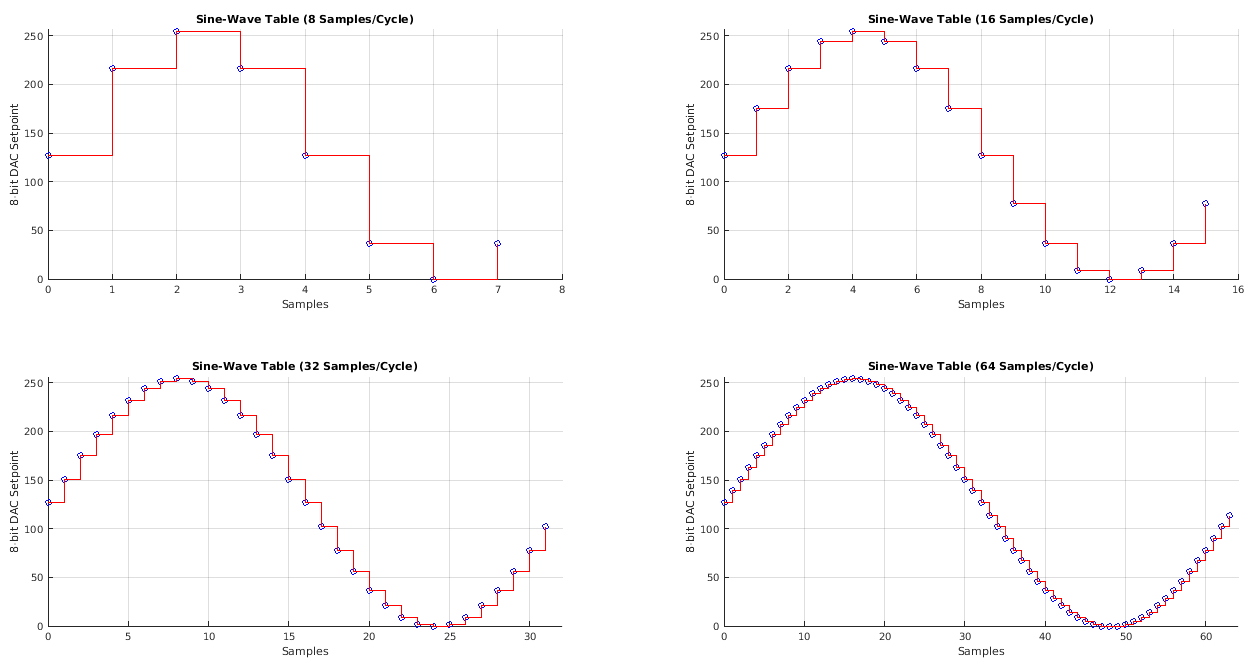
\includegraphics[width=\textwidth]{samples_sine}
    \caption{Sine-wave cycle under different sampling rates.}
    \label{samples_sine}
\end{figure}

 In order to get a good quality representation of an analog signal you'll need to have sufficient quantization resolution and sampling frequency. 
 
\subsection{Representing Analog Signals in Software} 
 Through quantization, analog signals can be represented in software as a list of numerical values. Part of the in-lab assignment uses a \textit{wave table} containing a digital representation of a single wave cycle. These tables are arrays, indexed by a counter that increments as the data is moved into the DAC. The rate at which the waveform samples are fed into the DAC determines the resulting output frequency. Figure \ref{wave_tables} contains the c-code for tables of the basic wave types.
 
 
%\smallskip
% \colorbox{gray!20!white}{
%     \parbox{\linewidth-2\fboxsep} {
%         \centering 
%         \lstinputlisting[language=C]{./Files/wave_tables.c}
%     }
% }
% 
%\smallskip
 
\code{./Files/wave_tables.c}{Wave tables used in the lab assignment.}{wave_tables}
 
Figure \ref{wave_tables} shows graphs of each table in figure \ref{wave_tables}. These tables use 8-bit data (256 quantization levels) with 32 samples per wave cycle. Increasing the number of samples per cycle would improve the smoothness of the output. However, increasing the number of samples also requires a much higher rate of moving data into the DAC to achieve the same output wave frequency. 

This lab will use the main application loop to move data from a wave tables to the DAC peripheral. A more refined approach could use a timer interrupt or the direct-memory-access peripheral (DMA). 

\begin{figure}[]
    \centering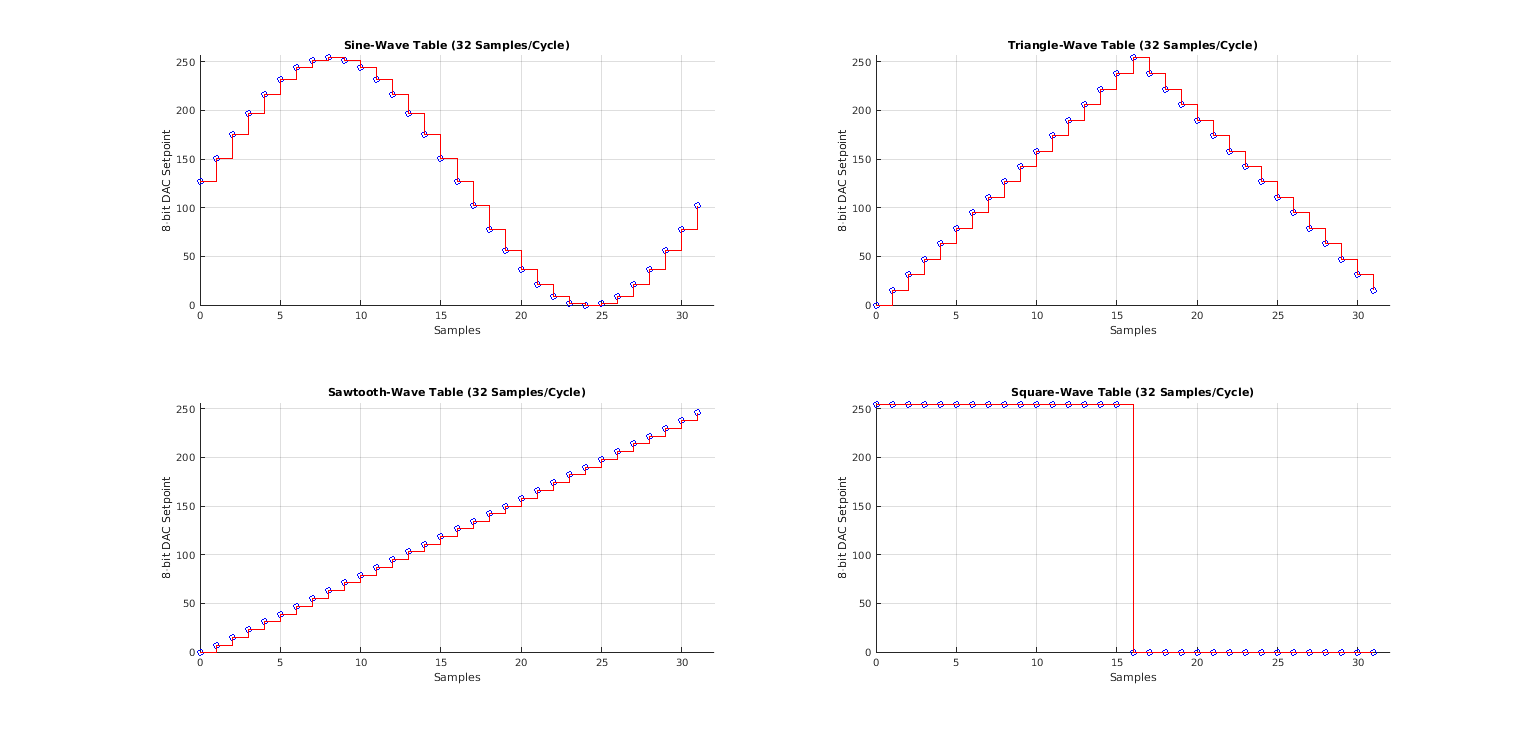
\includegraphics[width=\textwidth]{wave_tables}
    \caption{Graphical representation of the wave tables used in the lab assignment.}
    \label{wave_tables}
\end{figure}
 
%\section{Analog Input/Output Sources}
%\subsubsection{Voltage Dividers}
%There are a number of ways to get a variable analog voltage. One of the easiest is to use a circuit called a voltage divider. A voltage divider is two resistors in series that are placed between two different voltages. (for example 3V and GND) By changing the resistance ratio between the two resistors it is possible to generate any voltage in the range between the two endpoints. The following equation shows the behavior of a voltage divider:
%
%\begin{equation*}
%    V_{out}\:=\frac{\:R_2}{R_1+R_2}\cdot V_{in}
%\end{equation*}
%
%Instead of placing two separate resistors and then swapping them out to change the output voltage, we'll be using a device called a potentiometer. A potentiometer is a three-terminal device that is essentially a long resistor with a movable "tap" or connection in the middle. By adjusting the dial on the top of the device the tap moves along between the resistive material in the potentiometer and the resistance between it and each of the endpoints changes. 
%
%\begin{figure}[]
%    \centering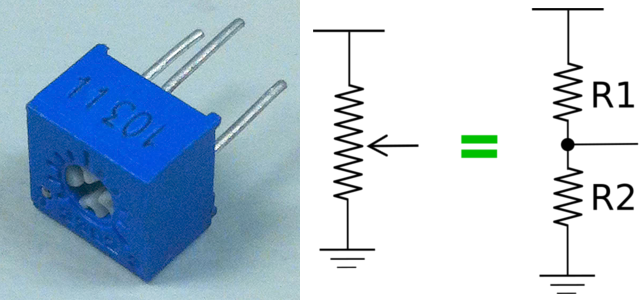
\includegraphics[width=.5\textwidth]{pot}
%    \caption{Potentiometer used as a voltage divider.}
%    \label{pot}
%\end{figure}
%
%Potentiometers are excellent for building voltage dividers because they look exactly like a pair of resistors in series. By adjusting the location of the tap, the ratio of the resistors changes and you get a different analog voltage on the tap pin.
%
%For this lab you'll want to use jumper wires to connect one of the end of the potentiometer to 3V and the other to GND. The center (tap) pin will be the analog voltage output, you'll need to connect that to whatever pin you are using as the ADC input.  
 
\section{The Analog to Digital Converter (ADC)}
Similarly to the USART the analog-to-digital converter of the STM32F0 is a remarkably powerful and flexible peripheral. The on-chip 12-bit successive approximation (SAR) ADC has 19 multiplexed measurement channels of which 16 are connected to external pins and the others measuring internal peripherals and sensors. The ADC can be configured to scan enabled channels in a variety of patterns and conversions are either triggered by hardware events (such as a timer update event) or the ADC can be configured to continuously run. See section 13.4.8 in the peripheral reference manual for information about the ADC's operational modes. 

The output of the ADC can be configured into a few different bit-width's depending on the conversion time, storage capacity and resolution requirements of the user application. The ADC can output data in either 12-bit, 10-bit, 8-bit or 6-bit resolution. As the output resolution decreases, the amount of time required for each analog conversion drops.

\subsection{Peripheral Registers}
Because there are delays between starting a conversion cycle and getting an output, the ADC uses status flags throughout all its registers to notify the user when it is ready to start a new conversion, when it is busy, what input in a conversion sequence is currently active and more. There are many advanced modes and features that we won't be using for this lab, you will have to look through the registers and ignore things that don't look like they are needed for the assignment requirements. The main registers you will need for this lab are mentioned here.

\subsubsection{ADC Interrupt and Status Register (ADC\_ISR)}
The interrupt and status register contains interrupt flags as well as a few high-level status bit which indicate when the ADC is ready for use. 

\subsubsection{ADC Control Register (ADC\_CR)}
The ADC control register is used to startup, calibrate, and shutdown the ADC peripheral. 

To minimize errors due to voltage offset and drift, it is important that you allow the ADC to perform a self-calibration process every time you first turn it on. Additionally the ADC has a warm-up period after you enable it before you can start a conversion process. 

\begin{warning}
    One common source of confusion when first using the ADC is that many of the bits in the control register are not only used to control the peripheral, but are also modified by hardware as status flags. 
      
    An example of this is the self-calibration. Once the user triggers a calibration cycle by setting the appropriate bit, the ADC will clear that same bit when calibration is complete. Most of the bits in the control register have strict requirements for when the ADC will allow you to set them. You will need to read the bit descriptions to know what you are allowed to configure before/after each step.
\end{warning}    

\subsubsection{ADC Configuration Register 1 (ADC\_CFGR1)}
The configuration register sets the operational mode, data resolution, and trigger source of the ADC. 

\subsubsection{ADC Channel Selection Register (ADC\_CHSELR)}
Each input to the ADC has a conversion channel associated with it. The channel selection register controls which of these channels are read by the ADC when operating. You will need to enable the channel associated with the input pin you choose in the lab assignment. 

\subsubsection{ADC Data Register (ADC\_DR)}
The data register holds the most recently converted value. You will read the quantized value of the ADC input pin from this location. 

\subsection{Initializing the ADC}
This section will list the basic procedure of calibrating, enabling, and starting the ADC without mentioning the actual flags and conditions for advancement. For details on the specific bits and flags to modify, use sections 13.4.1 (Calibration) and 13.4.2 (ADC on-off control) in the peripheral reference manual.

To initialize the ADC for use:
\begin{enumerate}
    \item Set the desired operating mode, data resolution, and trigger source. 
    \begin{itemize}
        \item Single conversion mode performs one measurement every time the ADC is triggered. Continuous conversion mode repeatedly measures and updates the data register. 
        \item The trigger source selects whether software or a hardware signal starts a new conversion process. 
    \end{itemize}
    \item Start the ADC calibration
    \begin{itemize}
        \item Calibration can only be performed when the peripheral is stopped, don't set any enable/start bits (other than in the RCC peripheral) before attempting to start a calibration process. 
    \end{itemize}
    \item Wait for the hardware to signal that the calibration has completed.
    \begin{itemize}
        \item The ADC will clear the calibration start/request bit when the process has completed. 
    \end{itemize}
    \item Set the peripheral enable.
    \item Wait until the ADC ready flag is set. 
    \item Start the ADC conversion.
    \begin{itemize}
        \item Starting a conversion sequence is separate from enabling the peripheral. 
        \item Since the lab assignment uses continuous conversion mode, this bit only needs to be set once at the beginning. 
    \end{itemize}
\end{enumerate}

\section{The Digital to Analog Converter (DAC)}
In contrast to the ADC, the digital-to-analog converter is one of the simplest peripherals to configure on the STM32F0. It can have either one or two output channels (the STM32F072 has two) with either 8 or 12-bit operation. After configuration, you only need to write a value into the appropriate data register and the DAC will automatically update to the analog representation of that value.


\subsection{Peripheral Registers}

\subsubsection{DAC Control Register (DAC\_CR)}
The DAC control register selects the trigger source and enables/disables the output channels. The trigger source of the DAC determines whether software (writing to a data holding register) causes the DAC to update its output, or if the peripheral waits on a signal from a peripheral such as a timer.  

\subsubsection{Data Holding Registers}
The DAC has three different types of data holding registers used depending on the desired data format. When triggered, the DAC moves the data from the appropriate holding register into the read-only output registers. 

The three possible operation modes are:
\begin{itemize}
    \item \textbf{DAC\_DHR8Rx} -- 8-bit right-aligned (data in bits 0-7)
    \item \textbf{DAC\_DHR12Rx} -- 12-bit right-aligned (data in bits 0-11)
    \item \textbf{DAC\_DHR12Lx} -- 12-bit left-aligned (data in bits 15-4)
\end{itemize}

The left-aligned mode is typically used for selecting the upper bits of a 16-bit number, allowing the DAC to act on 16-bit data without any conversion or shifting. (with some minor loss in precision provided by low-order bits) You can read more about the DAC's data formats in section 14.5 of the peripheral reference manual.

\subsection{Initializing the DAC}
There are only two steps to initializing the DAC for use:
\begin{enumerate}
    \item Set the trigger source for the channel/output update.
    \item Enable the channel used for output. 
\end{enumerate}

\section{Analog Functions of GPIO Pins}
Similar to the alternate function system which connects pins to digital signals within the chip, the STM32F0 has an analog bus that connects pins to internal analog peripherals. 

For this lab we want to connect a couple of pins to \textit{ADC\_INx} (ADC input) and \textit{DAC\_OUTx} (DAC output) signals. 

\subsubsection{Finding a Pin's Analog Functions}
Open the STM32F072 chip datasheet to chapter 4 - \textit{Pinouts and pin descriptions}. Because we're dealing with chip specific pin routing, we can't get the information we need directly from the GPIO peripheral. Take a look at table 13, you'll notice that it maps pin names such as PA0 to physical package pin numbers as well as specifying input/output characteristics, alternate functions and additional functions.

Scan through the table looking at the additional functions available for the GPIO pins. Find PB0 and examine it, hopefully you'll notice that its additional function is ``ADC\_IN8'' one of the ADC input channels. Figure \ref{analog_pins} shows a portion of table 13 with the analog functions of PB0 highlighted.

\begin{figure}[]
    \centering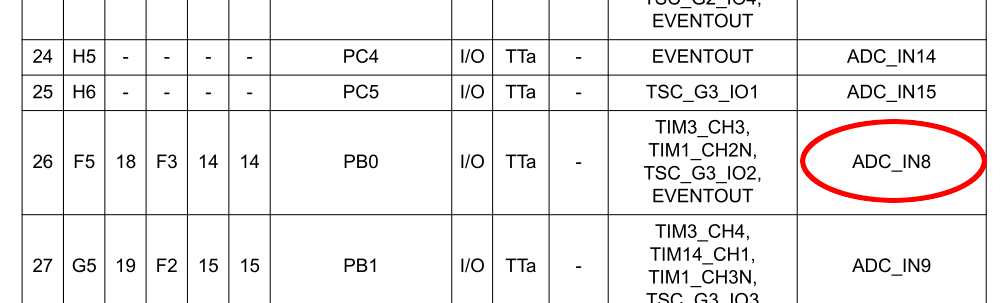
\includegraphics[width=\textwidth]{analog_pins}
    \caption{Section of table 13 with analog functions of PB0 highlighted.}
    \label{analog_pins}
\end{figure}

\subsubsection{Setting a Pin's Additional (Analog) Function}
Unlike the alternate function system the analog bus on the STM32F0 isn't configurable. Pins are permanently assigned analog functions and beyond setting the GPIO peripheral to analog mode there isn't any additional configuration required. Setting a pin to analog mode disconnects it from the GPIO peripheral, this means that the other GPIO settings such as output speed or type don't have any effect.

\section{Lab Assignment}
The exercises in this section introduce the basic operation of the ADC and DAC peripherals. Each exercise is standalone, however they can be implemented together in the main application loop without conflict. 
%These peripherals are usually used as a component of a larger signal-processing system, the final exercise is optional 
\subsection{Measuring a Potentiometer With the ADC}
The goal of this exercise is to use the ADC to measure the position of a potentiometer and display the result using the LEDs on the Discovery board. Each LED will have a threshold voltage/value that will cause it to turn on if the measured output of the ADC is greater. Likewise, they should turn off if the value drops below the threshold. When the potentiometer is turned so that the output (center) pin's voltage increases, the LEDs should light up in sequence. \\ 

\textbf{Your lab TA should have potentiometers available for use during the lab session.} For out-of-lab use, you can purchase small potentiometers from the lab stockroom. The potentiometers for sale typically require a small screwdriver to adjust and jumper wires or breadboard to connect to the Discovery board. 

\begin{enumerate} 
    \item Initialize the LED pins to output.
    \item Select a GPIO pin to use as the ADC input.
    \begin{itemize}
        \item Check 
        \item Remember that the ``ADC\_INx'' additional/analog function indicates which ADC input channel the pin connects to.
        \item Configure the pin to analog mode, no pull-up/down resistors.
        \item Connect the output (center pin) of a potentiometer to the input pin. The other two pins of the potentiometer should be connected to 3V and GND.
    \end{itemize} 
    
    \begin{warning}
        
    \end{warning}

    \item Enable the ADC1 in the RCC peripheral. 
    \item Configure the ADC to 8-bit resolution, continuous conversion mode, hardware triggers disabled (software trigger only).
    \item Select/enable the input pin's channel for ADC conversion.
    \item Perform a self-calibration, enable, and start the ADC.
    \begin{itemize}
        \item The lab manual describes the basic procedure without mentioning the actual flags and conditions for advancement. 
        \item Use sections 13.4.1 (Calibration) and 13.4.2 (ADC on-off control) in the peripheral reference manual. 
    \end{itemize}
    \item In the main application loop, read the ADC data register and turn on/off LEDs depending on the value.
    \begin{itemize}
        \item Use four increasing threshold values, each LED should have a minimum ADC value/voltage to turn on.
        \item As the voltage on the input pin increases, the LEDs should light one-by-one.
        \item If the pin voltage decreases below the threshold for a LED, it should turn off. 
    \end{itemize}
\end{enumerate}



\subsection{Generating Waveforms with the DAC}
The goal of this exercise is to generate an analog waveform that can be viewed using either an oscilloscope or the analog input of a Saleae logic analyzer. The DAC peripheral will be fed values from one of the lab wave-tables located in figure \ref{wave_tables}.

\begin{enumerate}
    \item Select a GPIO pin to use as the DAC output.
    \begin{itemize}
        \item Remember that the ``DAC\_OUTx'' additional/analog function indicates which DAC output channel the pin connects to. 
        \item Configure the pin to analog mode, no pull-up/down resistors.
        \item Connect an oscilloscope probe or channel 0 of a Saleae logic analyzer to the pin.
        \begin{itemize}
            \item Remember that the old Saleae 16's available for checkout do not have analog capabilities. Unless you have a new-model logic analyzer, you will need to use an oscilloscope. 
        \end{itemize}    
    \end{itemize}
    \item Set the used DAC channel to software trigger mode. 
    \item Enable the used DAC channel. 
    \item Copy one of the wave-tables in figure \ref{wave_tables} into your application. 
    \begin{itemize}
        \item The wave tables are 32-element arrays of unsigned 8-bit values.
        \item Don't use the square-wave. Pick one of the sine, triangle, or sawtooth waveforms. 
    \end{itemize}
    \item In the main application loop, use an index variable to write the next value in the wave-table (array) to the appropriate DAC data register. 
    \begin{itemize}
        \item Use the one that matches closest to the value type of the wave-table.
    \end{itemize}
    \item Use a 1ms delay between updating the DAC to new values. 
    \begin{itemize}
        \item The resulting frequency of the waveform will be: \\ \textit{1 kHz (1ms between updates) / 32 samples per cycle $\approx$ 31 Hz}
    \end{itemize}
    \item Submit a screen capture or photograph of the oscilloscope or logic capture in your postlab.
\end{enumerate}
\end{document}
